%%%%%%%%%%%%%%%Conjectures regarding values of Riemann zeta function at Gram points%%%%%%%%%%%%%%%%%%%%%%%%%%%%%%%%%%%%%%%%%%%%%%%%%%%%%%%%%%%%%
%

\documentclass[twoside]{article}
\usepackage{graphicx}
\usepackage{amsmath,amsthm,amssymb,verbatim}
\usepackage{fancyhdr}
\pagestyle{fancy}
\usepackage{url}

\def\blfootnote{\xdef\@thefnmark{}\@footnotetext} 
\long\def\symbolfootnote[#1]#2{\begingroup%
\def\thefootnote{\fnsymbol{footnote}}\footnote[#1]{#2}\endgroup} 

\newtheorem{mydef}{Conjecture}

\setcounter{page}{1}
\begin{document}

\date{}
\lhead[]{}
\chead[\underline{xxx}]{\it{ updated April 30 2017}}
\rhead[]{}

\title{\bf{Conjectures regarding Riemann zeta function at Gram points}}


\author{O. Shanker 
 \thanks{Mountain View, CA 94041, U. S. A. Email: oshanker@gmail.com
 }
}

\maketitle
\thispagestyle{fancy}

\begin{abstract}
Riemann's hypothesis is one of the key unsolved problems which is attracting
a lot of attention. 
Researchers are making extensive numerical studies of the location of the 
zeta function zeros to complement the theoretical work. 
The evaluation of the zeta function at large heights involves time consuming
calculations. The values of the 
zeta function at Gram points plays an important role in the computations. In 
this work we present two conjectures about the distribution of zeta values at the 
the Gram points. We present quantitative evidence for the conjectures.
\end{abstract}


\symbolfootnote[0]{\bf{April 2017}}


\clearpage
\chead[\underline{O. Shanker}]{\underline{Conjectures regarding Riemann zeta function at Gram points}}


\section{Introduction}
Riemann's hypothesis about the location of 
the roots of the Riemann zeta function is a key unsolved problem in mathematics,
which challenges us to this day. The study also has ramifications in physics and
random matrix theory. 
There is an impressive body of empirical evidence for his hypothesis,
but a formal proof has been elusive. The numerical studies have found
regions where the hypothesis is almost violated, but no counter-example has
been found. The numerical evaluation of the zeros is time-consuming, and the values of the 
zeta function at Gram points plays an important role in the computations~\cite{korolev1,korolev2}.  The behavior at the Gram points also provides good features for  Machine Learning applications to the study of the Riemann zeta zeros \cite{osneural,osentropy}.  In 
this work we present two conjectures about the distribution of zeta values at the 
the Gram points. These conjectures are most likely related to the symmetry properties of the rotated zeta function (Hardy's function) under inversion around the origin. We present quantitative evidence for the conjectures. 

\begin{mydef}\label{antisymmetry}
(even-odd antisymmetry): The distribution of the zeta values for odd Gram points is the negative of the distribution of zeta values for the even Gram points.
\end{mydef}
\begin{mydef}\label{symmetry}
(forward-backward symmetry): When we consider a sequence of zeta values at consecutive Gram points, the properties of the sequence are symmetric with respect to the direction of the sequence of Gram points (i.e., the sequence behaves similarly whether we consider the points in increasing order or in decreasing order).
\end{mydef}

The paper is organized as follows.
Section~\ref{sec2} establishes the required notation for the 
Riemann Zeta Function. 
Section~\ref{sec3} describes the numerical evaluation of the Riemann zeta function. 
Section~\ref{sec4} presents the statistics of the zeta value distributions for different types of Gram points and compares the predictions of the two conjectures with the actual results from the numerical evaluations.. 
Section~\ref{conclusions}
gives a brief summary of the results. 


\section{\label{sec2}Theory of zero distributions of Riemann zeta function }

In this section we  establish the required notation for the 
Riemann Zeta Function. 
The Riemann Zeta function is defined for $\mathrm{Re} (s) > 1$ by
\begin{equation}
\zeta ( s ) \, = \, \sum^{\infty}_{n = 1} \; n^{-s} \, = \, \prod_{p \in primes} \;
\left( 1 - p^{-s} \right)^{-1}.
\label{eqRie}
\end{equation}

Eq.~(\ref{eqRie})  converges for $\mathrm{Re} (s) > 1$.  
 $\zeta ( s )$ has a  continuation
to the complex plane and satisfies a functional equation \cite{Riemann(1858),Riemann(1892),Titchmarsh(1986),Edwards(1974)}
\begin{equation}  
\xi(s):= \pi^{-s/2} \, \Gamma (s/2) \, \zeta ( s ) \, = \, \xi ( 1 - s );
\label{eq:func}
\end{equation}
$\xi(s)$ is entire except for simple poles at $s = 0$ and $1$. Riemann
multiplied the definition by $s(s-1)$ to remove the poles. We
write the zeroes of $\xi(s)$ as $1/2 + i \gamma$. The Riemann Hypothesis  
asserts that $\gamma$ is real for the non-trivial zeroes.
We order the $\gamma$s in increasing order, with 
\begin{equation}
\ldots \ldots \gamma_{-1} \, < \, 0 \, < \, 
\gamma_1 \, \leq \, \gamma_2 \ldots. 
\end{equation}
Then $\gamma_j \, = \, - \gamma_{-j}$ for $j = 1, 2, \ldots,$ 
and    $\gamma_1$, $\gamma_2$, $\ldots$  are roughly
$14.1347$, $21.0220$, $\ldots$.


Asymptotically, for the Riemann zeta function the mean number of 
zeros with height less than $\gamma$ (the smoothed Riemann zeta staircase)
is~\cite{Edwards(1974)}
\begin{equation}  
<\mathcal{N_R} (\gamma)> = (\gamma/2\pi)(ln(\gamma/2\pi)-1)-\frac{7}{8}.
\label{eq:Rnumber}
\end{equation}
Thus, the mean spacing of the zeros at height $\gamma$ is 
$2\pi(\ln (\gamma/2\pi))^{-1}$. For the range of $t$ values
studied by us this spacing is essentially constant at $0.2436$.

The study of the zeroes of the Riemann zeta function and Generalized 
Zeta functions is of interest to mathematicians and physicists. Mathematicians 
study the spacings because of its applications to analytic number theory, 
while physicists study it because of its  relation 
to the theory of the spectra of random matrix theories (RMT) 
and the spectra of classically chaotic quantum systems. 
Many remarkable properties of the Riemann zeta function keep turning up in the literature~\cite{os6,Matiyasevich}.


The next section gives the details of the numerical calculations.

\section{\label{sec3}Numerical Calculations}

In this section we discuss the details of the numerical work. 
The numerical analysis takes advantage of the functional 
equation Eq.~(\ref{eq:func}).
One defines
\begin{equation}
\theta(t) = arg (\pi^{−it/2} \Gamma(\frac{1}{4} + \frac{it}{2})), 
\label{eq:theta}
\end{equation}
where the argument is defined by continuous variation of $t$ starting with the value $0$ at $t = 0$.
For large $t$ $\theta$ has the asymptotic expansion
\begin{equation}
\theta(t) = \frac{t}{2}\ln (\frac{t}{2\pi}) - \frac{t}{2} - \frac{\pi}{8} + \frac{1}{48t} - \frac{1}{5760t^3}. 
\label{eq:thetaAsymptotic}
\end{equation}
A consequence of the zeta functional equation is that the function 
$Z(t)=exp(i\theta(t))\gamma(1/2 +it)$,
known as the Riemann-Siegel Z-function, is real valued for real $t$. 
Moreover we have $|Z(t)| = |\zeta(1/2+it)|$. Thus the zeros of $Z(t)$ are the imaginary part of the zeros 
of $\zeta(s)$ which lie on the critical line. We are led to finding the change of sign 
of a real valued function 
to find zeros on the critical line. This is a very convenient property in the numerical verification 
of the Riemann Hypothesis.
Another very helpful property is that many of the zeros are separated by the
"Gram points".  When $t \ge 7$, the $\theta$ function Eq.(\ref{eq:theta}) is monotonic increasing. 
For $n \ge 1$, the $n-th$ Gram point $g_n$ is defined as the unique solution $> 7$ to
$\theta (g_n) = n\pi$.
The Gram points are as dense as the zeros of $\zeta(s)$ but are much more regularly distributed.
Their locations can be found without any evaluations of the Riemann-Siegal series Eq.(\ref{eq:RS}).
Gram's law is the empirical observation that $Z(t)$ usually changes its sign in each Gram interval 
$G_n = [g_n,g_{n+1})$. 
This law fails infinitely often, but it is true in a large proportion of cases.
The average value of $Z(g_n)$ is $2$ for even $n$ and $-2$ for odd $n$~\cite{Titchmarsh(1986)},
and hence $Z(g_n)$ undergoes an infinite number of sign changes.


The Riemann-Siegel Z-function is evaluated using the Riemann-Siegal series
\begin{equation}
Z(t) = 2\sum^{m}_{n=1}\frac{\cos(\theta(t) - t \ln (n))}{\sqrt{n}} + R(t), 
\label{eq:RS}
\end{equation}
where $m$ is the integer part of $\sqrt{t/(2\pi)}$, and $R(t)$ is a small remainder
term which can be evaluated to the desired level of accuracy. The most important 
source for loss of accuracy at large heights is the cancellation between
large numbers that occur in the arguments of the $\cos$ terms in Eq.~(\ref{eq:RS}). We 
use a high precision module to evaluate the arguments. The rest of the calculation
is done using regular double precision accuracy. See ~\cite{hiary,gourdon,Odlyzko(1989)} for methods to efficiently evaluate the zeta function at large t.
We calculated the zeta function at a million Gram points starting at $t = 10^{12}$.

In the next section we present the statistics of the zeta value distributions for different types of Gram points. We compare the predictions of the two conjectures with the actual results from the numerical evaluations.

\section{\label{sec4}Statistics of the distribution}


\begin{figure*}
\centering
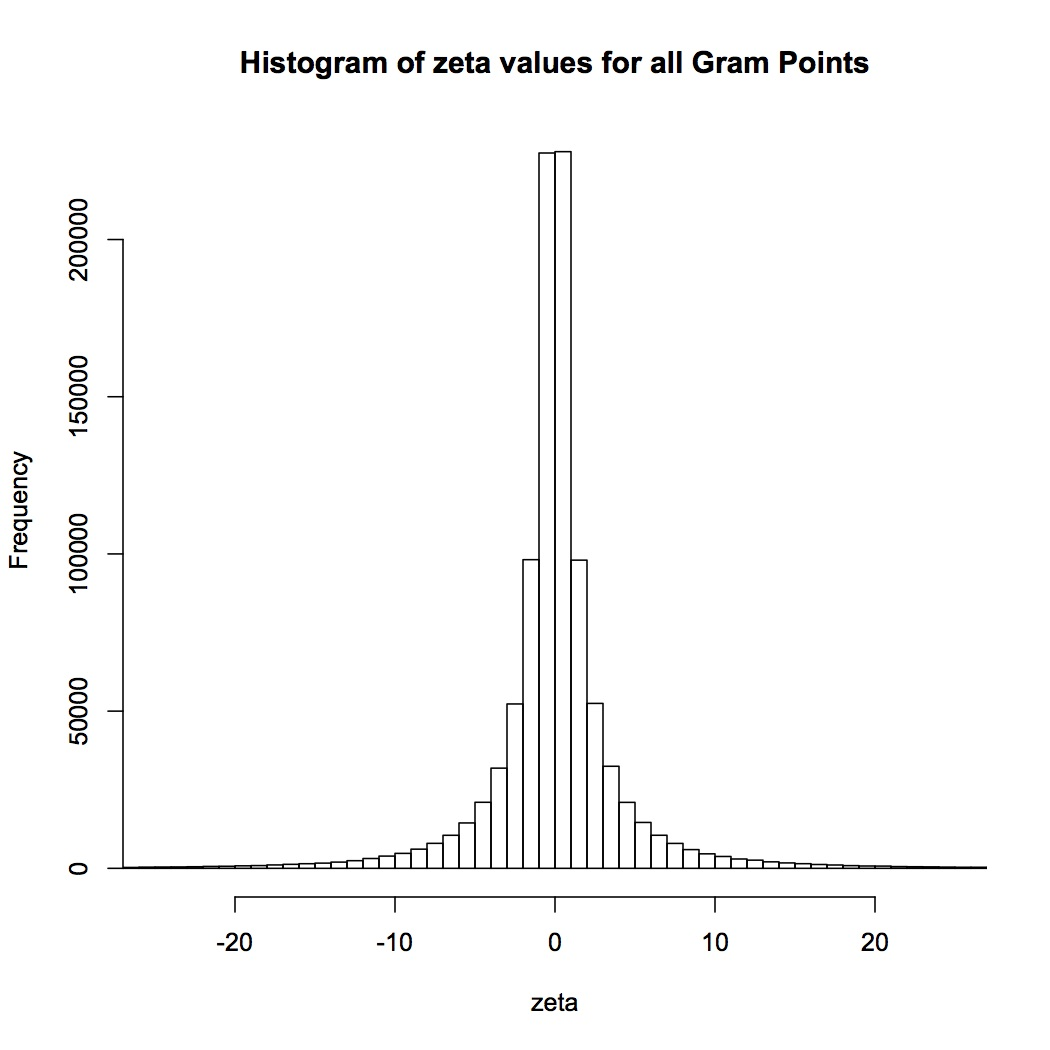
\includegraphics[width=0.62\textwidth]{rzeta.jpg}
\caption[]{ 
 Distribution of zeta values at a million Gram points starting at $t = 10^{12}$.
  }
\vspace{1mm}
\label{allhist}

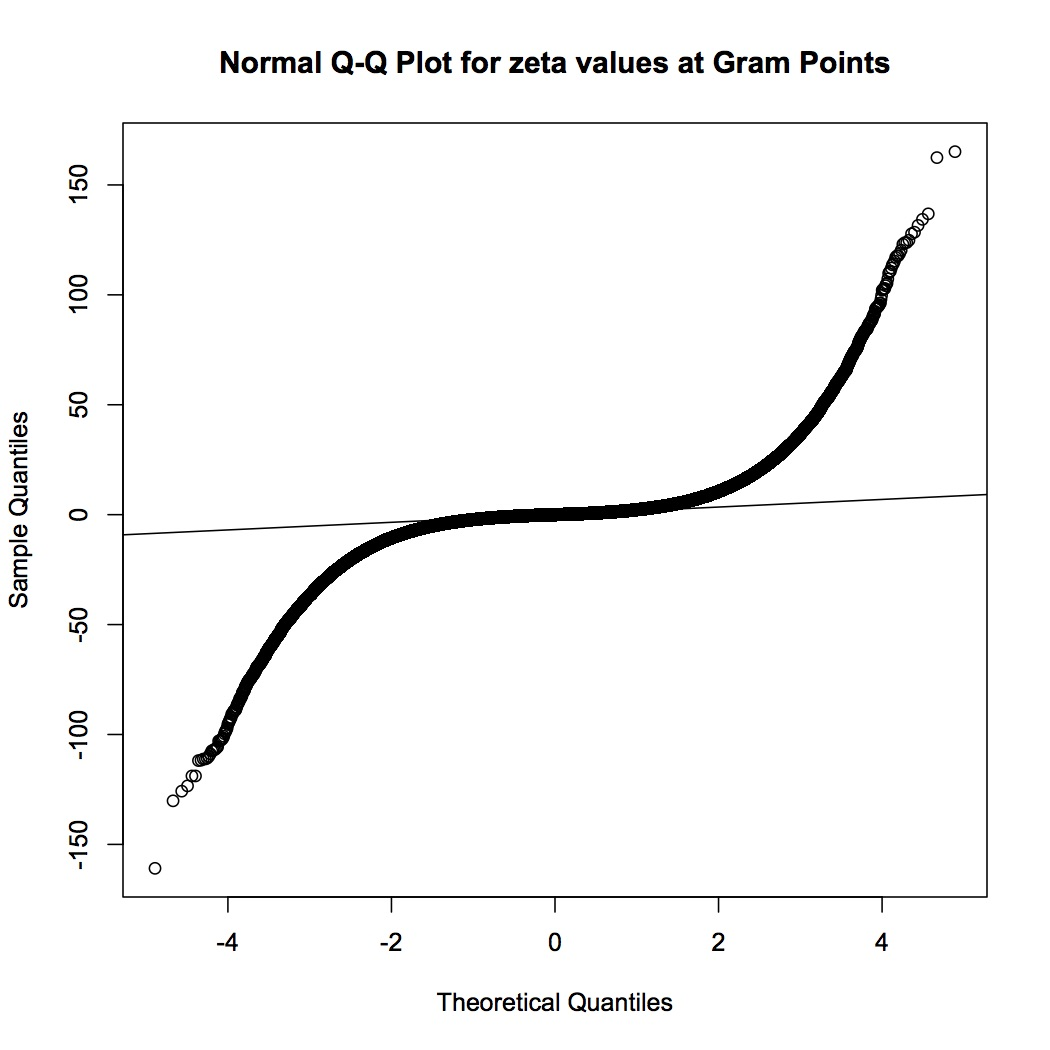
\includegraphics[width=0.62\textwidth]{qqr.jpg}
\caption[]{ 
 QQ plot of zeta values at a million Gram points starting at $t = 10^{12}$.
  }
\vspace{1mm}
\label{qqr}
\end{figure*}

\begin{table}
\centering \(\begin{array}{ccccccc}
\hline
 Gram &     Min.   & 1st    &  Median    &   Mean   & 3rd    &   Max. \\
 type &              & Quantile   &            &              & Quantile.    &   \\
\hline
All& -160.90 &   -1.17 &    0.00106 &   0.00  &  1.172 &165.10\\
Odd&-160.90 &   -2.526 &   -0.8471  & -2.00 &   -0.1121 &  69.41 \\
Even&-68.63 &   0.1139 &  0.8526  & 2.00 &   2.541 & 165.10 \\
\hline
\end{array}\)
\caption{Quantiles and mean for zeta values at Gram points of different types.} \label{tab:quantiles}
\end{table}

In this section we present the statistics of the zeta value distributions for different types of Gram points (all Gram points, odd Gram points and even Gram points). We present the relationships between the statistics that would be implied by Conjectures \ref{antisymmetry} and \ref{symmetry}, and we compare the predictions of the two conjectures with the actual results from the numerical evaluations. 

Figure~\ref{allhist} shows the histogram of zeta values for all Gram points. It  is symmetric around $0$. However, Figure~\ref{qqr}, the QQ plot, shows that the distribution is not normal. The distribution has a sharp peak and a long tail at extreme values of the zeta function. For even Gram points $80\%$ of the zeta values are positive, while for odd Gram points $80\%$ of the zeta values are negative. Table~\ref{tab:quantiles} presents the quantiles and mean for zeta values at Gram points of different types.  One can see good evidence that the odd and even distributions are mirror images of each other within expected statistical significance. In sections 
\ref{sec4a} and \ref{sec4b} we will present further statistical properties of zeta values at pairs and triples of consecutive Gram points. These will help to validate Conjectures  \ref{antisymmetry} and  \ref{symmetry}. In Section~\ref{sec4c} we present evidence for  Conjecture  \ref{symmetry} from Gram block counts.

\subsection{\label{sec4a}Conjecture 1}

\begin{figure*}
\centering
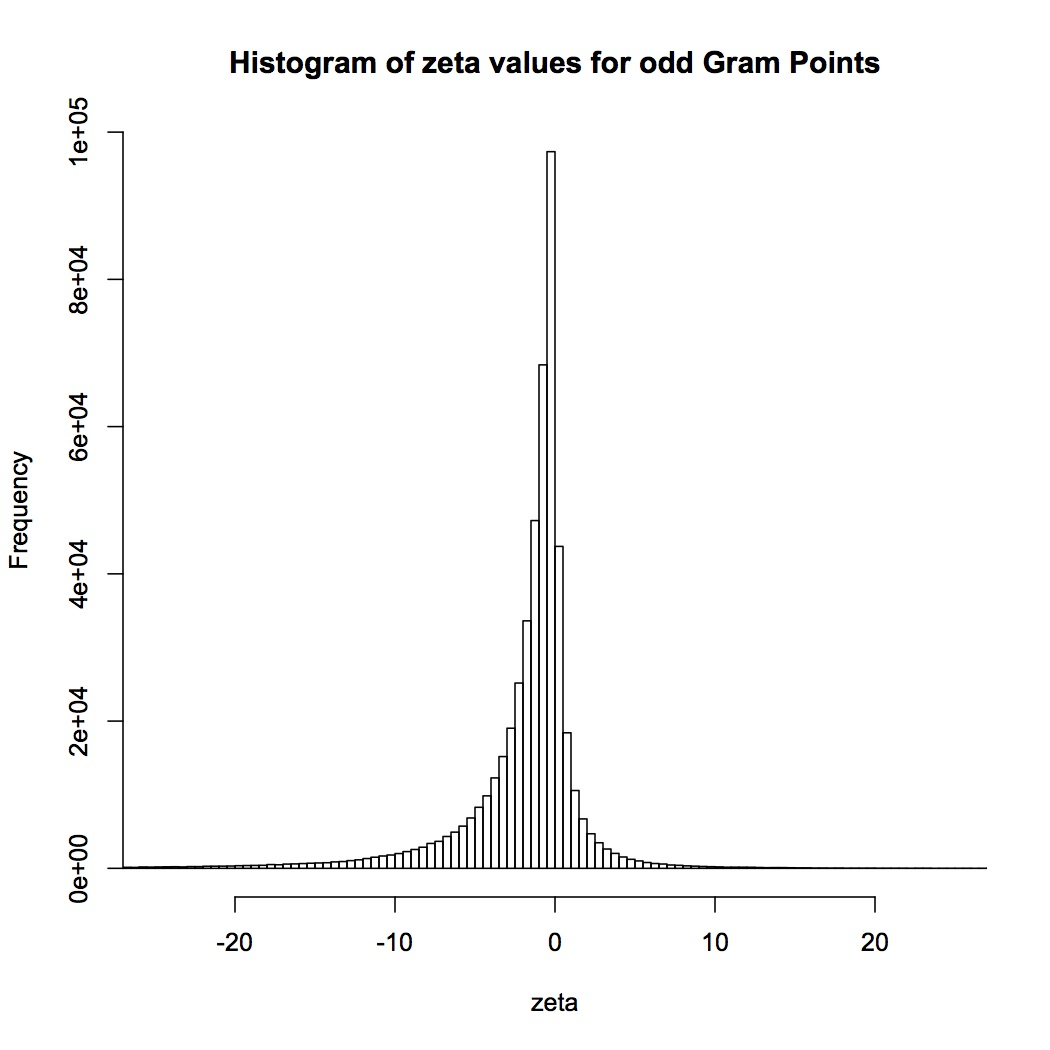
\includegraphics[width=0.62\textwidth]{ozeta.jpg}
\caption[]{ 
  Distribution of zeta values at 500000 odd Gram points starting at $t = 10^{12}$.
 }
\vspace{1mm}
\label{oddhist}

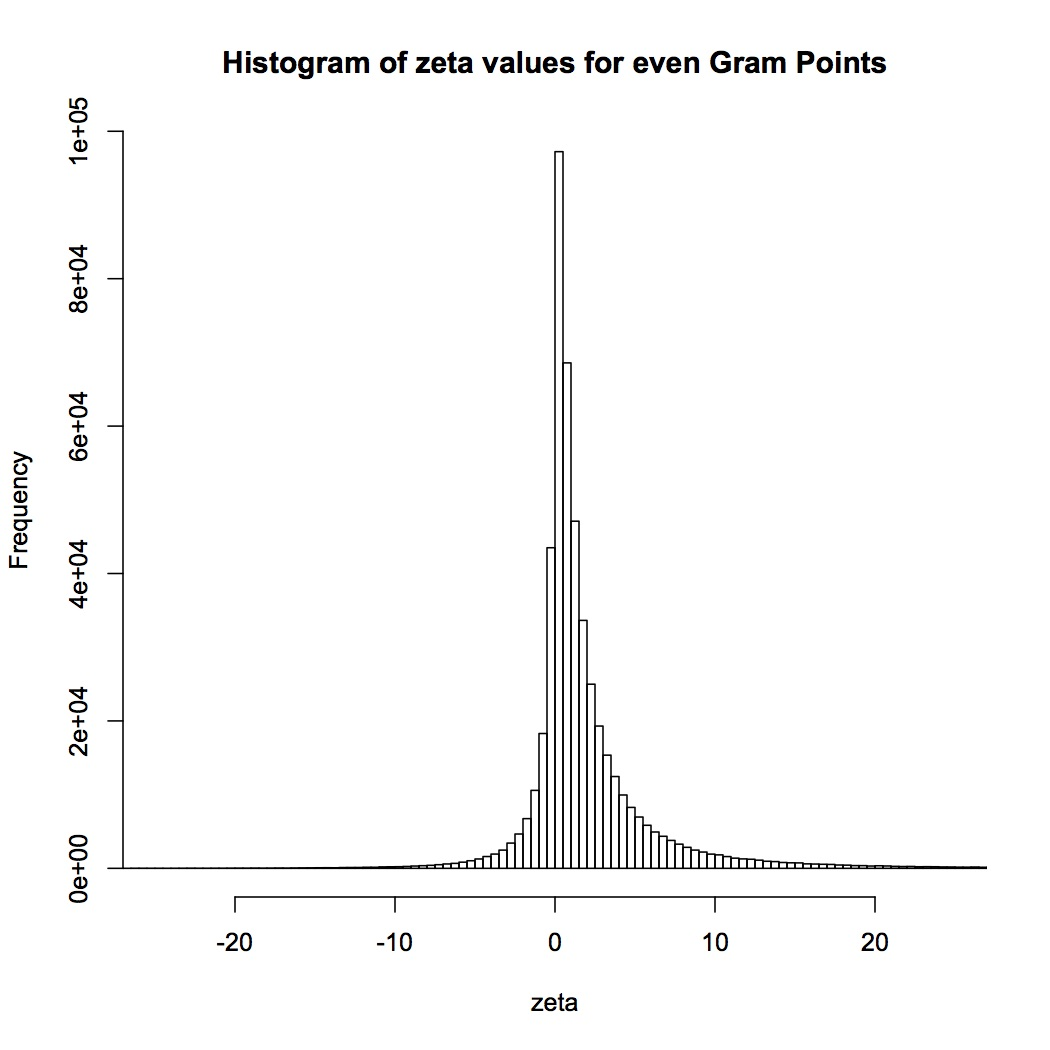
\includegraphics[width=0.62\textwidth]{ezeta.jpg}
\caption[]{ 
   Distribution of zeta values at 500000 even Gram points starting at $t = 10^{12}$.
 }
\label{evenhist}
\vspace{1mm}
\end{figure*}

In this section we will consider the statistics of zeta values at pairs of consecutive Gram points. We will look at the evidence for Conjecture \ref{antisymmetry}. 

Figures \ref{oddhist} and ~\ref{evenhist}  present the histograms of zeta values at odd Gram points and even Gram points respectively. These figures further bear out the evidence of Table~\ref{tab:quantiles} that the odd and even distributions are mirror images of each other. To study Conjecture \ref{antisymmetry} further, we will consider the zeta values at pairs of consecutive Gram points. We will classify the zeta values into two classes, '$+$' for positive zeta values ($zeta > 0$) and '$-$' for negative zeta values ($zeta \leqslant  0$). Thus, for example, the notation '$++$' stands for a Gram Point which has a positive zeta value followed by a Gram Point which has a positive zeta value, while the notation '$+-$' stands for a Gram Point which has a positive zeta value followed by a Gram Point which has a negative zeta value. Table~\ref{tab:pairraw} shows the counts for different pair configurations, for pairs beginning at odd Gram points (row 1) and for pairs beginning at even Gram points(row 2). Conjecture \ref{antisymmetry} predicts that the count for a configuration from the odd Gram point row in the table  will match the count for the mirror configuration in the even Gram point row of the table ( e.g., the count for '$++$' from the distribution for odd Gram points will match count for '$--$' from the distribution for even Gram points). Table~\ref{tab:pairtest} tests this prediction. The agreement is good, within the expected statistical variations. 

One might think that the all Gram points distribution can be used to verify Conjecture \ref{symmetry} by checking that the count for a given configuration  matches the count for the reversed configuration ( e.g., the count for '$+-$'  matches the count for '$-+$'). However, this equality follows just from count arguments, so there is no real test of Conjecture \ref{symmetry}.

\begin{table}
\centering \(\begin{array}{ccccc}
\hline
 Gram~type&   --   & -+   & +-   & ++  \\
\hline
Odd & 73117& 324793& 28590& 73501 \\
Even & 73309& 28398& 324600& 73693 \\
\hline
\end{array}\)
\caption{Counts of different configurations of zeta values for pairs of consecutive Gram points.} \label{tab:pairraw}
\end{table}

\begin{table}
\centering \(\begin{array}{ccccc}
\hline
 Gram~type&   --   & -+   & +-   & ++  \\
\hline
Odd & 73117& 324793& 28590& 73501 \\
\hline
Corresponding& 73693 & 324600 & 28398& 73309\\ 
Even~Entry     & (++)     & (+-)   & (-+)  & (--) \\
\hline
\end{array}\)
\caption{Test of Conjecture \ref{antisymmetry} using pairs of consecutive Gram points.} \label{tab:pairtest}
\end{table}


\subsection{\label{sec4b}Conjecture 2}
In this section we will consider the statistics of zeta values for triples of consecutive Gram points. We will look at the evidence for  Conjecture \ref{symmetry}.

\begin{table}
\centering \(\begin{array}{c|cccccccc}
\hline
 Gram~type&   ---   & --+       & -+-      & -++   &   +--      & +-+   & ++-   & +++ \\
\hline
 All &   66317& 80109& 272707& 80483& 80109& 273081& 80483& 66711\\
\hline
Counts~relationship&66317& 80109& 272707& 80483& 80109& 273081& 80483& 66711\\
prediction                            &  ---    & +--    & -+-       & ++-  & --+  & +-+ & -++ & +++  \\
\hline
\end{array}\)
\caption{Configurations of triples satisfy various equalities, even without Conjecture \ref{symmetry}.} \label{tab:tripletest}
\end{table}

\begin{table}
\centering \(\begin{array}{c|cccccccc}
\hline
 Gram~type&   ---        & --+       & -+-          & -++          &   +--           & +-+   & ++-   & +++ \\
\hline
Odd & 52717& 20400& 264789& 60003& 20592& 7998& 59811& 13690 \\
\hline
 &maps~to& 20592& maps~to& 59811& 20400& maps~to& 60003& maps~to \\ 
prediction   &  self         & +--       &  self        & ++-       & --+       & self        & -++      & self  \\
\hline
\hline
Even & 13600& 59709& 7918& 20480& 59517& 265083& 20672& 53021 \\
\hline
 &maps~to& 59517& maps~to& 20672& 59709& maps~to& 20480& maps~to \\  
prediction   &  self         & +--       &  self        & ++-       & --+       & self        & -++      & self  \\
\hline
\end{array}\)
\caption{Test of Conjecture~\ref{symmetry} for  even and odd Gram points.} \label{tab:tripletestcomplexity}
\end{table}


Using just counts based arguments, one can show that the count for a given configuration from the all Gram points distribution  will match the count for the reversed configuration ( e.g., the count for '$++-$' will match count for '$-++$'). Table~\ref{tab:tripletest} shows the relationship. There is no real test of Conjecture \ref{symmetry}.
Table~\ref{tab:tripletestcomplexity} shows that for the even and odd Gram points separately the agreement with the prediction of Conjecture~\ref{symmetry} is at the $1\%$ level. .

\subsection{\label{sec4c}Conjecture 2 and Gram Block}

\begin{table}
\centering \(\begin{array}{cc}
\hline
Length~of 	& Ratio  \\
Gram~block	& Type~II/Type~I \\
\hline
2& 0.999966866\\
3& 0.999941442\\
4& 0.999913803\\
5& 0.999871412\\
6& 0.999822002\\
7& 0.999594807\\
8& 0.999257121\\
9& 1.001677139\\
10& 0.992668154\\
\hline
\end{array}\)
\caption{Test of prediction of Conjecture \ref{symmetry} from Gram block counts.} \label{tab:rosser}
\end{table}

\begin{table}
\centering \(\begin{array}{cc}
\hline
Type~of~violation &Ratio~of~counts\\
\hline
2L3/2R3 &0.999651352\\
2L22/2R22 &0.999806111\\
3L3/3R3 &0.999217106\\
2L212/2R212 &0.999160495\\
3L22/3R22 &0.999640429\\
4L3/4R3 &0.998017358\\
2L2112/2R2112 &0.998100056\\
2L032/2R230 &0.999734774\\
3L212/3R212 &0.995621266\\
4L22/4R22 &0.998245284\\
2L04/2R40 &0.998111916\\
\hline
\end{array}\)
\caption{Forward-backward symmetry in patterns of violations of Rosser's rule.} \label{tab:vrr}
\end{table}

In this section we present the prediction of  Conjecture \ref{symmetry} on the distribution of different types of Gram blocks. We will follow the notation of  \cite{gourdon}.
A Gram point $g_n$ is called good if $(-1)^nZ(g_n) > 0$, and bad otherwise. A Gram block is an interval [gn, gn+k) such that $g_n$  and $g_{n+k}$ are good Gram points 
and $g_{n+1}, . . ., g_{n+k-1}$ are bad Gram points. A Gram block is denoted by the notation $a_1a_2 . . . a_k$ where k is called the length of the Gram block, and $a_i$ denote the number of roots of Z(t) in the Gram interval $[g_{n+i-1}, g_{n+i})$. So far, no Gram interval has been found with more than 5 zeros, thus the notation is unambiguous. $a_1$ and $a_k$ must be even while  $a_2$ to $a_{k-1}$ are odd.

A Gram block of length k which contains exactly k roots of Z[t) is called regular. The first and last Gram intervals of a regular Gram block must contain an even number of roots (0 or 2 roots). The internal Gram intervals must all contain an odd number of roots (all of them must contain one root if the end intervals contain 2 and 0 roots. If the end intervals both contain no roots, then one of the internal intervals must contain 3 roots.) 
Thus, Regular Gram blocks must have a pattern of one of the following three forms:
$21 . . . 10, 01 . . . 12, 01 . . . 131 . . . 10$
where the notation $1 . . . 1$ refers to any string of consecutive 1s, including the zero length string. Gourdon~\cite{gourdon} denotes these three types of regular Gram Blocks as Type I, Type II and Type III respectively. A simple generalization of Conjecture \ref{symmetry} above predicts that the number of Type I and Type II Gram blocks up to a given large height must be equal to each other (except for Type I Gram blocks of length one, which only have the pattern 1).  Table~\ref{tab:rosser}  (based on data in \cite{gourdon}) shows the ratio of counts of Gram Blocks of Type II to Type I, found up to $t = 10^{13}$. The prediction of Conjecture 2 is borne out to a remarkable degree, While there is very good evidence for the forward-backward symmetry from the ratio of Type II to Type I counts, there is another intriguing pattern: the Type II counts are ever so slightly smaller than the Type I counts. Thus, while we have a symmetry, it is broken very slightly.

Further validation comes from a consideration of the different types of violations of Rosser's rule~\cite{gourdon}, which also show the forward-backward symmetry. Rosser's rule states that Gram blocks of length $k$ contain at least $k$ zeros. This law is violated infinitely often, but is violated only for a small fraction of the Gram Blocks. A Gram block is either regular, or it has an excess of zeros, or it has fewer zeros than its length. The last type of Gram block violates Rosser's rule. 
If a Gram block of length k is an exception to Rosser's rule, then its pattern of zeros must be of the form $01...10$. To describe the exception, we must specify where the two missing zeros are. Gourdon uses the notation $kXa_1a_2 . . . a_m, X = L~or~R $ 
to describe an exception on a Gram block of length $k$  where the missing zeros are on the left (for $X = L$) or on the right (for $X = R$), the pattern containing the missing zeros being $a_1a_2 . . . a_m$ (moreover, this pattern is the smallest union of Gram block adjacent to the exception that contains the missing zeros). For example, $3L04$ denotes a violation of Rosser's rule on a Gram block of length 3, the missing zeros being at its left. Written out in detail, the pattern of zeros is expressed by the notation is $04010$.

The notation above classifies the type of violation of Rosser's rule, the value $m$ being called the length of the excess block. The notation used for exceptions to Rosser's rule is not unambiguous. When several contiguous violations of Rosser's rule exists, they may overlap or missing zeros can be in the same Gram interval. Such situations are very rare, and in these cases (Gourdon found just three occurrences until the $10^{13}th$ zero), Gourdon uses the notation $Ma_1 ...a_l$ where the pattern $a_1 . . . a_l$ is made of the minimal contiguous Gram blocks containing at least one violation to Rosser rule, and all the missing zeros. For example, the pattern $M00500$, first encountered at gram index $n = 3,680,295,786,518$, denotes a situation with two violations of Rosser's rule ($00$ and $00$, Gram blocks with missing zeros) and a single Gram interval containing all the missing zeros (pattern $5$). 
Table~\ref{tab:vrr}  (based on data in \cite{gourdon}) shows the forward-backward symmetry in patterns of violations of Rosser's rule. Once again, while there is very good evidence for the forward-backward symmetry, the $L$ type violations are ever so slightly smaller than the $R$ type violations. Again, we have evidence for a symmetry which is broken very slightly.

\section{\label{conclusions}Conclusions}

In this work we presented two conjectures regarding the distribution of zeta function values at Gram points. The conjectures refer to the even-odd Gram Point antisymmetry and the forward-backward symmetry ("time reversal" symmetry, if we think of the zeta values at Gram points as being a time series). After briefly describing the theory of the Riemann zeta function and the numerical evaluation, we presented statistics of the zeta function values. The statistics provide validation for the two conjectures.

 
\begin{thebibliography}{10} 

\bibitem{korolev1} Maxim Korolev,
"GRAM'S LAW AND THE ARGUMENT
OF THE RIEMANN ZETA FUNCTION", Publications de Institut Mathmatique,
\url{http://elib.mi.sanu.ac.rs/files/journals/publ/112/n106p053.pdf}, (2012)

\bibitem{korolev2} Maxim Korolev,
"On small values of the Riemann zeta-function at Gram points", Sbornik: Mathematics,
\url{http://iopscience.iop.org/article/10.1070/SM2014v205n01ABEH004367/meta},
{\bf205}, (2014)

\bibitem{osneural} O. Shanker, ``Neural Network prediction of Riemann zeta zeros''
{\it Advanced Modeling and Optimization}, {\bf 14}, 717-728, (2012). 

\bibitem{osentropy} O. Shanker, ``Entropy of Riemann zeta zero sequence''
{\it Advanced Modeling and Optimization}, {\bf 13}, 449-456, (2013). 

\bibitem {Riemann(1858)} B. Riemann, ``\"{U}ber die Anzahl der Primzahlen uter
Einer Gegebenen Gr\"{o}be,'' {\it Montasb. der Berliner Akad.}, (1858),
671-680.

\bibitem {Riemann(1892)} B. Riemann, ``Gesammelte Werke'', Teubner, Leipzig, (1892).

\bibitem {Titchmarsh(1986)} E. Titchmarsh, ``The Theory of the Riemann Zeta
Function,'' Oxford University Press, Second Edition, (1986).

\bibitem {Edwards(1974)} H. M. Edwards, ``Riemann's Zeta Function,'' 
Academic Press,  (1974).

\bibitem{os6} O. Shanker, 
"Generalised Zeta Functions and Self-Similarity of Zero Distributions",
{\it J.  Phys. A} {\bf39}(2006), 13983-13997.

\bibitem {Matiyasevich} Y. Matiyasevich, 
"An artless method for calculating approximate values of
zeros of Riemann zeta function",
Web report, \url{http://logic.pdmi.ras.ru/~yumat/
personaljournal/artlessmethod/artlessmethodtexts.php}, (2013)

\bibitem{hiary} G. A. Hiary,
"METHODS TO COMPUTE THE RIEMANN ZETA
FUNCTION", arxiv.org, math.NT, 0711.5005v4, (2011).

\bibitem{gourdon} Xavier Gourdon,
"The $10^{13}$ first zeros of the Riemann Zeta function,
and zeros computation at very large height", report,
\url{http://numbers.computation.free.fr/Constants/Miscellaneous/zetazeros1e13-1e24.pdf}, (2004)

\bibitem {Odlyzko(1989)} A. Odlyzko, ``The $10^{20}$-th Zero of the Riemann Zeta
Function and 70 Million of its Neighbors,'' (preprint), A.T.T., (1989).

\end{thebibliography} 

\end{document} 

